
\documentclass[tikz,border=8pt]{standalone}
\usepackage{amsmath}
\usepackage{xcolor}
\usetikzlibrary{arrows.meta,positioning,calc,shapes.geometric}
\definecolor{Canvas}{HTML}{FAF9F6}
\definecolor{Ivory}{HTML}{FFFFF0}
\definecolor{Divider}{HTML}{E5E5EA}
\definecolor{Gold}{HTML}{C5A059}
\definecolor{WarmGold}{HTML}{D4AF37}
\definecolor{SoftPink}{HTML}{FBEFEF}
\definecolor{Ink}{HTML}{2C2C2E}
\tikzset{decision/.style={rectangle,draw=Gold,line width=1.2pt,fill=Canvas,minimum width=1.5cm,minimum height=1cm,align=center,text=Ink},chance/.style={circle,draw=WarmGold,line width=1.2pt,fill=Ivory,minimum size=1.45cm,align=center,text=Ink},payoff/.style={regular polygon,regular polygon sides=3,shape border rotate=90,draw=Gold,line width=1.2pt,fill=SoftPink,minimum size=1.25cm,align=center,text=Ink},branch/.style={draw=Ink,line width=0.9pt,-{Latex[length=2mm]},line cap=round},chosenbranch/.style={draw=Gold,line width=1.15pt,-{Latex[length=2mm]},line cap=round},callout/.style={rectangle,rounded corners=5pt,draw=Divider,fill=Ivory,text=Ink,align=center,inner sep=6pt}}

% Asset ID: OffSpecDecisionAnalysisTikZ-001
% Source: transcripts.md, Decision Analysis 1
% Purpose: Provide a precise LaTeX/TikZ decision-tree notation key.
\begin{document}
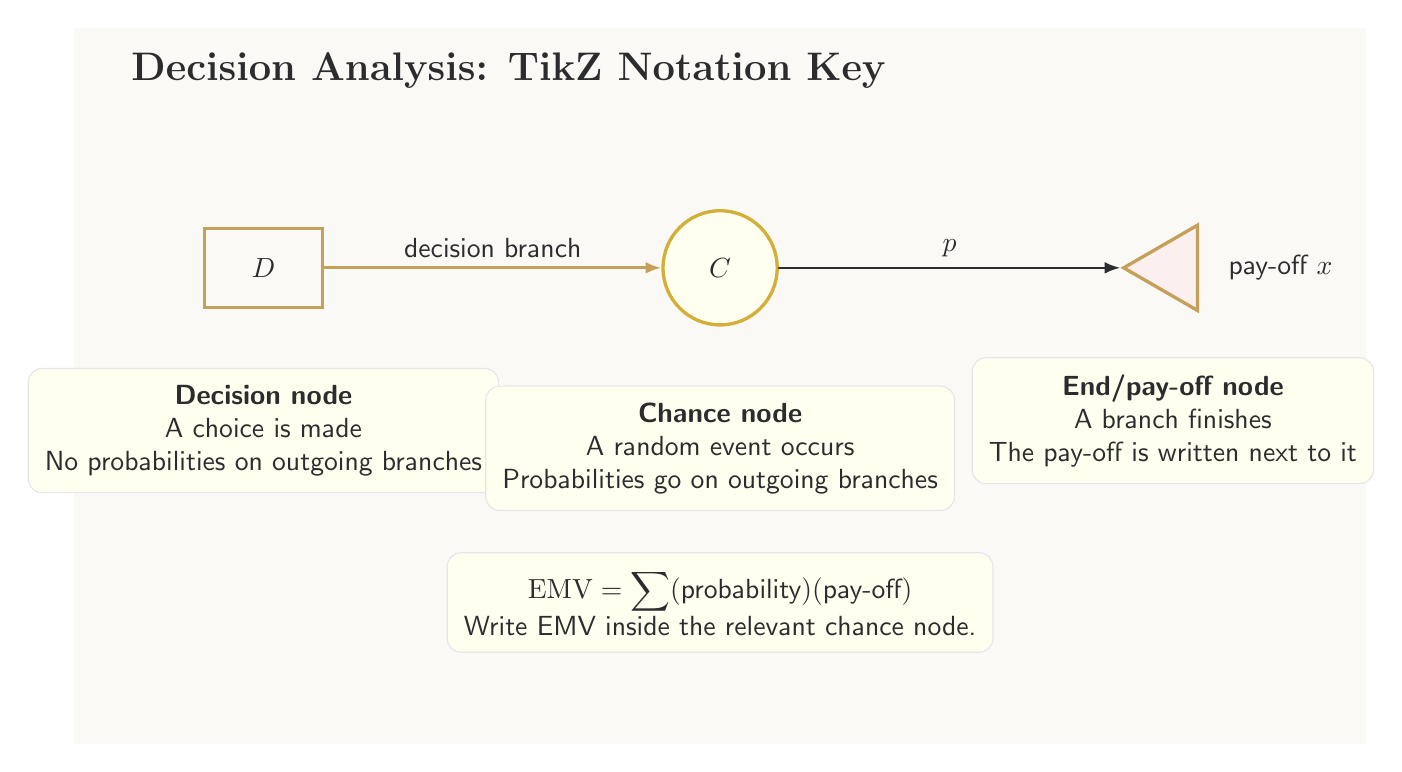
\begin{tikzpicture}[font=\sffamily]
\fill[Canvas] (-0.6,-0.7) rectangle (15.8,8.4);
\node[anchor=west,text=Ink,font=\bfseries\Large] at (0,7.85) {Decision Analysis: TikZ Notation Key};
\node[decision] (D) at (1.8,5.35) {$D$};
\node[callout, below=0.75cm of D] {\textbf{Decision node}\\A choice is made\\No probabilities on outgoing branches};
\node[chance] (C) at (7.6,5.35) {$C$};
\node[callout, below=0.75cm of C] {\textbf{Chance node}\\A random event occurs\\Probabilities go on outgoing branches};
\node[payoff] (P) at (13.35,5.35) {};
\node[callout, below=0.75cm of P] {\textbf{End/pay-off node}\\A branch finishes\\The pay-off is written next to it};
\draw[chosenbranch] (D) -- node[above,sloped,text=Ink] {decision branch} (C);
\draw[branch] (C) -- node[above,sloped,text=Ink] {$p$} (P);
\node[anchor=west,text=Ink] at ($(P.east)+(0.25,0)$) {pay-off $x$};
\node[callout] at (7.6,1.1) {$\displaystyle \operatorname{EMV}=\sum (\text{probability})(\text{pay-off})$\\Write EMV inside the relevant chance node.};
\end{tikzpicture}
\end{document}
